\newgeometry{left=3.7cm, right=3.7cm,bottom=4cm} %, top=3cm}
\chapter[Neutral MSSM Higgs Bosons Search]{Search for neutral MSSM Higgs Bosons in  
$A/h/H \rightarrow \tau^{+}\tau^{-} \rightarrow e \mu + 4\nu$ decays} \label{chap:anal}


%
 \vspace{0.5cm}

%A search for neutral MSSM Higgs bosons with the ATLAS detector at the
%LHC is presented.  This analysis is based on an integrated luminosity of $20.3 ~fb^{-1}$
%of proton-proton collisions at a centre-of-mass energy of 8 TeV. 
%
%The analysis focusses on the decay of neutral Higgs bosons into a pair of tau
%leptons, which subsequently decay to an electron, a muon and four
%neutrinos. Furthermore, 
%
In light of the recent discovery of a Higgs 
boson with mass of $\sim 126$ GeV at the LHC~\cite{AHiggsO,CHiggsO}, it remains an open question
whether this new particle is the only missing piece of the electroweak symmetry breaking
sector or whether it is one of several Higgs bosons predicted in  theories 
that go beyond the SM. The most recent measurements \cite{ASpin0,ACouplings,CFermions,CWidth} of its
properties shows this new boson to be, within experimental uncertainties, fully
compatible with the SM Higgs boson. Nevertheless, such a new particle can also still
be accommodated within several theories beyond the 
standard model (BSM). Among all of them, Supersymmetry  is a theoretically favoured scenario
as the most predictive framework beyond the Standard Model.

This chapter presents the search for the neutral MSSM Higgs bosons decaying into pairs of tau leptons
in the fully leptonic final state, published in Ref.~\cite{}\footnote{to Sandra: I'll remove this sentence
if Conf note wont be ready in time} as a part of the search for the neutral
MSSM Higgs bosons in all final states of the tau leptons decay. 
The search is based on 20.3 $\text{fb}^{-1}$ of  data at a centre-of-mass energy of $\sqrt{s} = 8$~TeV
recorded by the ATLAS experiment during 2012.
This chapter is organised as follows: a brief summary of the MSSM Higgs sector 
and an introduction to the analysis strategy is given in Section~\ref{sec:intro},
while the event selection and categorization are described in Section~\ref{sec:selection}. 
Section~\ref{sec:BackgroundEstimation} describes the estimation of the backgrounds and
in Section~\ref{sec:Systematics} methods to evaluate systematic uncertainties are discussed. Finally, 
in section~\ref{sec:result}, an overview of the statistical methods employed along with the corresponding
result of the search are presented.

%There are two approach to explore the Higgs sector:
%one can study the coupling of the Higgs boson with vector
%bosons and fermions, those measure in fact are sensitive to new physics and can determine
%%given the unitarily property of scattering
%%amplitudes for longitudinal vectors and fermions, one can understand 
%if this particle is  fully responsible for
%the generation of all the SM particles masses. 
%Another approach is to directly search for %model dependent
%for additional Higgs es in a well defined model, which is the approach followed in this
%thesis where new neutral bosons are sought within the MSSM (see chapter \ref{}). 
%
%
%%Discovering the mechanism responsible for electroweak
%%symmetry-breaking and the origin of mass for elementary particles has been
%%one of the major goals of the physics program at the Large Hadron
%%Collider~(LHC)~\cite{LHC}.  In the Standard Model (SM) this mechanism
%%requires the existence of a single scalar particle, the Higgs
%%boson~\cite{ENGLERT,HIGGS,HIGGS2,HIGGS3,Guralnik:1964eu}.
%
%%This chapter is divided in three sections:
%%in section~\ref{sec:strategy} an introduction to experimental searches and to the strategy
%of this particular analysis is given, in section~\ref{sec:bkg} is described the core of this thesis
%work, i.e. the detail of the background modelling for this analysis, while in section~\ref{sec:result}
%the result of the search are presented.


\restoregeometry
\clearpage
\newpage

\section{Introduction } \label{sec:intro}

\subsection{The Higgs Sector in the MSSM}

\begin{figure}[tp]
     \begin{center}

            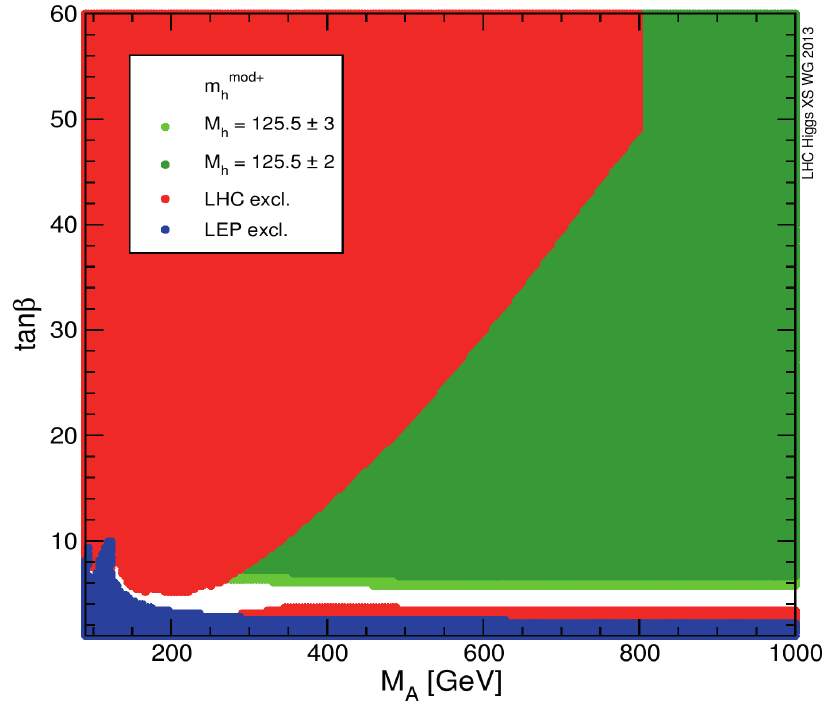
\includegraphics[width=0.7\textwidth]{figure/mh_mod.png}

    \end{center}
    \caption{Excluded and allowed regions of the $m_{A} - \text{tan}\beta$ parameter space for the  $m_{h}^{mod+}$ 
	MSSM benchmark scenario. Excluded regions are determined based on direct Higgs boson searches at LEP 
	(blue) and LHC (red). The two green 
	bands correspond to the parameter regions which are compatible with the assumption that 
	the lightest MSSM Higgs boson, \emph{h}, has a mass respectively of $M_{h} = 125.5 \pm 2$ (dark green) 
	or $125.5 \pm 3$ GeV (light green). For more detail 
	see~\cite{LHCxsec}.}
   \label{fig:mhmod}
\end{figure}

In the Minimal Supersymmetric extension of the Standard Model
(MSSM)~\cite{MSSM1, MSSM2} the Higgs sector is composed of two Higgs
doublets of opposite hyper-charge, resulting in five observable Higgs
bosons:  two of these are neutral and $CP$-even
($h$,$H$), one is neutral and $CP$-odd ($A$) and two are charged
($H^\pm$).  At tree level their properties such as masses, widths and
branching ratios can be predicted in terms of only two parameters,
often chosen to be the mass of the $CP$-odd Higgs boson $m_A$ and
the ratio of the vacuum expectation values of the two Higgs doublets
$\tan\beta$ (for more details see chapter~\ref{chap:theory}).  
The MSSM predicts the existence of a Higgs boson with properties that  
resemble those of a SM Higgs boson in large regions of its parameter space. 
This is usually the case for the lightest Higgs boson, \emph{h}, while the other two, $H$ and $A$, 
tend to be degenerate in mass and decouple from gauge bosons.
%Production and decay mode 
%with vector bosons are forbidden for the CP-odd, $A$ and are suppressed for 
%the CP-even, $H$, Higgs bosons. 
On the other hand, the couplings of the latter two Higgs bosons with down (up) type fermions are enhanced
(suppressed) proportionally to the value of $\tan\beta$, meaning that for large $\tan\beta$
bottom-quark and $\tau$ lepton will play an important role for the Higgs bosons production and its decays. 
 
The two most relevant MSSM Higgs bosons production mechanisms 
at the LHC are gluon fusion, $gg\rightarrow A/H/h$, and 
the production in association with $b$-quarks, $pp \rightarrow b(b)A/h/H$, the latter becoming increasingly 
important for large values of $\tan\beta$. These two are the only production mechanisms
considered in this analysis. 
Assuming there are no decays into supersymmetric particles since these are too heavy, 
the favoured neutral MSSM Higgs bosons decay mode  is the decay into a pair of b-quark and anti-quark,
$A/h/H \rightarrow b\bar{b}$. This is followed, for the CP-odd $A$ and CP-even $H$ Higgs bosons, 
by the decay into pairs of $\tau$ leptons. Given that it is very difficult to distinguish the former decay 
from the large $b\bar{b}$ background, the decay mode 
$A/h/H \rightarrow \tau^+ \tau^-$  provides the highest sensitivity in the search for neutral MSSM Higgs bosons.

Searches for neutral MSSM Higgs bosons have been performed at
LEP~\cite{LEPLimits}, the
Tevatron~\cite{TevatronLimits1} and the LHC~\cite{CMSLimit, ATLASLimit}. 
In the following the search for the neutral MSSM Higgs bosons  in the final state 
$A/h/H \rightarrow \tau^+ \tau^- \rightarrow e \mu +4\nu$ is presented. 
This search is complementary to the searches in other $\tau^+\tau^-$ final states
characterised by the presence of one or two hadronicaly decaying $\tau$ leptons. Despite of the fact that the 
$\tau\tau$ branching ration in $e \mu +4\nu$ is only 6\%, this decay channel provides a sensitivity 
to the signal comparable to those in other $\tau\tau$ final states, especially for low $m_A$ values. 
This is mainly due to the high transverse momentum threshold at the trigger level for  hadronicaly decaying $\tau$ leptons.

As it is impractical for an experimental  search to explore the full parameter space of the MSSM, 
which has many free parameters, several benchmark scenarios are  
introduced by fixing all except $m_A$ and $\tan\beta$ parameters to values typical for most interesting 
physics cases.
With the recent Higgs boson discovery, benchmark scenarios of the MSSM have been updated to 
accommodate for  new experimental constraints. 
As an example, Figure~\ref{fig:mhmod} shows the currently excluded and allowed regions of the MSSM parameter space
for the  $m_{h}^{mod+}$ updated benchmark scenario. In this scenario a large region of the $m_{A} - \text{tan}\beta$
parameter space is compatible with the assumption that the observed Higgs boson correspond to the supersymmetric
CP-even neutral Higgs boson, $h$. A large part of this parameter space is still experimentally unexplored,
this is a strong motivation to pursue the search for additional neutral MSSM Higgs bosons.


\subsection{Signal and Background Processes}
Signal events in which the neutral MSSM Higgs bosons decay through 
$A/h/H \rightarrow \tau^+ \tau^- \rightarrow e \mu +4\nu$ process are characterised 
by the presence of one electron and one muon of opposite charge. These two leptons are isolated and have 
relatively high transverse momenta. In addition, four neutrinos contribute to the missing transverse energy in the event. 
Figure~\ref{fig:feyndiagSignal} shows leading order Feynman diagram for the two considered signal production modes,
gluon fusion and in association with $b$-quarks.
The presence (absence) of a b-jet in the final state serves as a main characteristic for the event categorization
in the latter (former) case, as described later on.

\begin{figure}[tp]
     \begin{center}
     \subfigure[]{		
            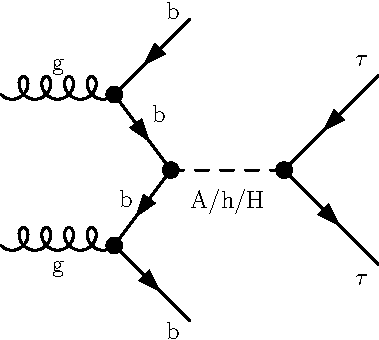
\includegraphics[height=3.5cm]{feyn_diagrams/diagrams/bbA.pdf}
     }\hspace{0.2cm}	
     \subfigure[]{		
            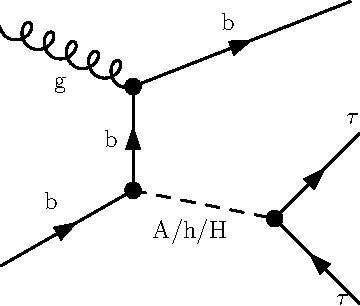
\includegraphics[height=3.5cm]{feyn_diagrams/diagrams/bbA2.pdf}
     }	\hspace{0.2cm}	
     \subfigure[]{		
            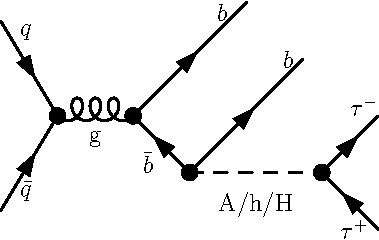
\includegraphics[height=3cm]{feyn_diagrams/diagrams/bbA3.pdf}
     }
     \subfigure[]{	
            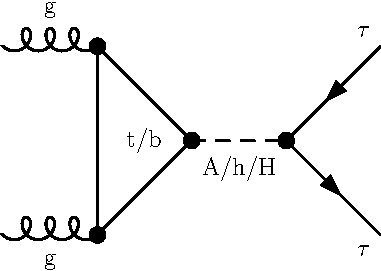
\includegraphics[height=3cm]{feyn_diagrams/diagrams/ggH.pdf}
	}	
     \end{center}
    \caption{Feynman diagram for the production of the neutral MSSM Higgs bosons in association with  $b$-quarks (a,b,c) and via gluon fusion (d) 
	process, subsequent decay in tau lepton pairs is considered.}
   \label{fig:feyndiagSignal}
\end{figure}

The described signal topology  is common to several other known SM background  processes which in general  
have higher cross sections than the sought signal.
The dominant background processes are the  $Z/\gamma^* \rightarrow \tau^+ \tau^- $ production
either via Drell-Yan process or in association with jets and the top quark production ($t\bar{t}$ and single top quark production ). 
Additional significant background contributions originate from the  dibosons production 
($WW$, $WZ$, $ZZ$) and QCD multi-jet events with non-prompt leptons  from hadron decay.
Vector boson production ($\Wlnu$ or $\Zll$, where $\ell \equiv e,\mu$)  in association with jets 
is also considered, but has small impact on the total background contamination. Examples of 
leading order Feynman diagrams for the dominant background processes are shown in Figure~\ref{fig:feyndiagBack}.
The production cross sections times the relevant branching fraction for signal and background processes are summarized in
Table~\ref{tab:MCxsec}. 
%The $W/Z$ and $b\bar{b}A/H/h$ production cross sections 
%are calculated to NNLO. The one for $\ttbar$, single top and dibosons cross sections are calculated at NLO.
%Finally, the direct $gg\rightarrow A/H/h$ signal cross sections 
%are calculated at NNLO and NLO for the top loop and the bottom loop respectively.
%

\begin{figure}[tp]
     \begin{center}
     \subfigure[]{		
            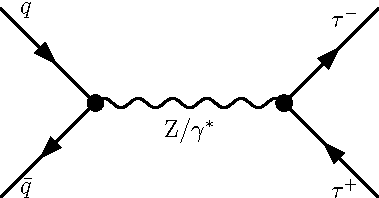
\includegraphics[height=3cm]{feyn_diagrams/diagrams/Ztautau.pdf}
     }\hspace{0.2cm}	
     \subfigure[]{		
            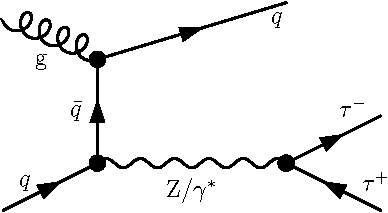
\includegraphics[height=3cm]{feyn_diagrams/diagrams/Z_plus_jet.pdf}
     }	
     \subfigure[]{		
            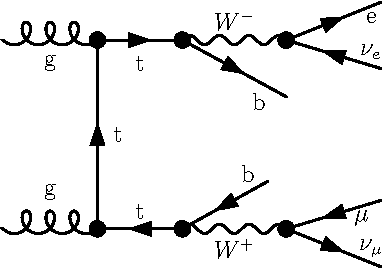
\includegraphics[height=3.5cm]{feyn_diagrams/diagrams/top.pdf}
     }\hspace{0.2cm}	
     \subfigure[]{	
            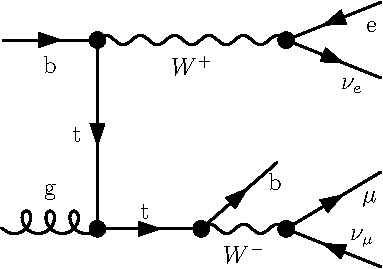
\includegraphics[height=3.5cm]{feyn_diagrams/diagrams/singletop.pdf}
	}	
     \subfigure[]{	
            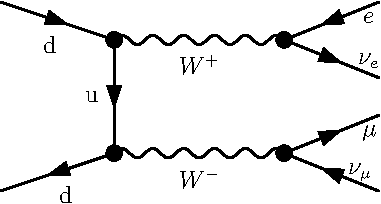
\includegraphics[height=3.2cm]{feyn_diagrams/diagrams/diboson.pdf}
	}\hspace{0.2cm}		
     \subfigure[]{	
            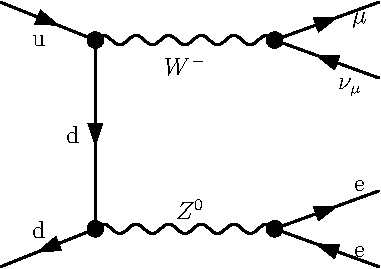
\includegraphics[height=3.2cm]{feyn_diagrams/diagrams/diboson2.pdf}
	}	
     \end{center}
    \caption{Examples of tree level Feynman diagrams for the production and decays of the most relevant backgrounds. The production of 
	 $Z/\gamma^* \rightarrow \tau^+ \tau^- $ either via Drell-Yan process or in association with jets  is shown in (a) and (b), top quark pair and
	single top quark production in (c) and (d), while examples of $WW$ and $WZ$ production are shown in (e) and (f) respectively.
	}
   \label{fig:feyndiagBack}
\end{figure}


%The values of the steering parameters used for the HERWIG, JIMMY and PYTHIA
%generators are described in Ref.~\cite{ATLASMC09Tune}.

\begin{table}[!tp]
\begin{center}
%\begin{footnotesize}
\begin{small}
\begin{tabular}{lr}
\hline \hline
Process                                                                 & Cross-section~(pb) [$\times$ BR] \\ [1pt]
\hline
\multicolumn{2}{c}{Signal ($m_A=150$~GeV, $\tan\beta=20$, $m_{h}^{mod}$ scenario) }  \\ [1pt]

$gg\rightarrow A/h/H \rightarrow\tau\tau \rightarrow e\mu+ 4\nu$                 &  $0.24 /0.20 / 0.95 $ \\
$pp \rightarrow b\bar{b}A/h/H \rightarrow \tau\tau \rightarrow e\mu + 4\nu$       & $0.53 /0.05 / 0.49   $ \\[1pt]
\hline
\multicolumn{2}{c}{Backgrounds} \\[1pt]
$W\rightarrow \ell \nu$+jets                           & 12.22$\times 10^3$ \\
$Z/\gamma^{*}\rightarrow \ell\ell$+jets       & 5.5$\times 10^3$ \\
$t\bar{t} \rightarrow \ell \ell + X$                                                              & 137.3 \\
Single top quark ($t-$, $s-$ and $Wt-$channels) $\rightarrow \ell + X$               & 28.4, 1.8, 22.4 \\
Dibosons (WW, WZ and ZZ ) $\rightarrow \ell \ell+ X$                                          & 20.6, 6.8, 1.55 \\ [1pt]
\hline 
\hline
\end{tabular}
\end{small}
\caption{The cross sections multiplied by the relevant branching ratios~(BR) for signal and the considered
background processes. The symbol $\ell$ stands for $\ell= (e, \mu, \tau)$. 
Signal cross sections are calculated for the $m_{h}^{mod}$ scenario assuming
 $m_A=150$~GeV and $\tan\beta=20$. The masses of the other two neutral MSSM Higgs bosons are 
	in this case  $m_H=151$~GeV and $m_h=125$~GeV.}
 \label{tab:MCxsec}

\end{center}
\end{table}


\subsection{Analysis Strategy} \label{sec:strategy}


In this thesis a search for the MSSM 
$A/h/H \rightarrow \tau^+ \tau^- \rightarrow e \mu +4\nu$ decays is presented. The $ee +4\nu$ and $\mu\mu +4\nu$ final states 
are not considered since a large background contribution is  expected  from $\Zee$ and $\Zmumu$ decays,  respectively, such that the sensitivity of the search in these final
state is significantly reduced.

Candidate events are selected based on the topological properties of the Higgs boson production
and decay. The  presence of exactly one electron and one muon is required in each event. Electron and muon are required to be 
 isolated and of opposite electrical charge.
The  events are categorized into two mutually orthogonal event categories. In the so called  \emph{b-vetoed} event category,
the absence of any b-tagged jets is required, thus searching mainly the signal produced via gluon fusion. The main background 
process in  this category is $\Ztautau$. 
In contrast, the presence of exactly one  b-tagged jet is required in the so called \emph{b-tagged} event category, 
searching predominantly signal produced in association with b-quarks. The requirement of a b-jet 
in the final state suppresses the $\Ztautau$ background, consequently, $\ttbar$ and single top quark  production
are the main background processes in this event category. Further selection criteria are introduced in both event categories, 
these are optimised to enhance the signal produced by the corresponding production mode.

The  search is performed within the MSSM $m_h^{mod}$ benchmark scenario
scanning the $m_A - \tan\beta$ plane in the ranges $90 \leq m_A \leq 300$ GeV and $5 < \tan\beta < 60$.
The prediction of the signal event yields and kinematical distributions are evaluated by simulation.
The contribution of the dominant $\Ztautau$ background process is measured in a dedicated  signal-depleted control data sample,
in order to reduce the systematic uncertainties of the simulation. Similarly, the QCD multi-jet background contribution 
is also estimated from dedicated data control sample since this background process it is hardly modelled by simulation.
%the large cross section puts high demands on the number of simulated events.
Contribution of  all  other background processes  is estimated from simulation.
The modelling of the background processes is  validated using different signal-depleted validation data samples and
good agreement is found.

The systematic uncertainties  on cross section calculations and the modelling of the detector response are
taken into account for simulated signal and background processes. For background processes  that are measured with  data,
the uncertainties of the corresponding measurement methods are evaluated.

The final statistical interpretation of the data is based on the 
comparison of the observed $\tau\tau$ invariant mass distributions with the prediction of the  background-only and signal-plus-background
hypothesis. Exclusion limits on the signal production are set by means of a binned profiled likelihood ratio
test statistic. The limits are interpreted  within the MSSM $m_{h}^{mod}$ scenario in terms of the constraints on the 
 $m_A$ and $\tan\beta$ values. Furthermore, the results are also expressed in a less model-dependent
way in terms of the upper limits on the cross section for the production of a generic Higgs boson $\phi$ with a  mass  $m_\phi$ 
via the production processes $pp \rightarrow b\bar{b}\phi$ and $gg \rightarrow \phi$.


 

%neutral MSSM Higgs bosons with the ATLAS experiment at CERN is
%presented, using proton-proton collisions at centre-of-mass energy of
%8~TeV, with a recorded integrated luminosity of
%$20.3 \ifb$.



\subsection{Data and Simulated Event Samples}
\label{sec:sample}
\subsubsection{Data Sample}

The  presented result  are based on proton-proton collision data
recordered by the ATLAS experiment during 2012 at a centre-of-mass energy of $\sqrt{s}=8$~TeV,
corresponding to an integrated luminosity of 20.3 fb$^{-1}$.
The events used in this analysis are recorded using a combination of a
single electron and combined electron-muon triggers. Only recorded events 
in which all  relevant components of the ATLAS detector were
fully operational are considered.
Additional data quality requirements are applied to each event according to~\cite{ATLASCLEANING}.
These requirements assure the rejection of  events %with data corruption due to the LAr and Tile calorimeters and
with jet activity in known noisy calorimeter regions. 




\subsubsection{Signal Samples}
%Both the signal and background process modelled by Monte Carlo (MC)
%simulation were produced within the ATLAS MC12a production campaign.
%The generators used for the different processes are described below.
Signal production via the gluon fusion process, $gg\rightarrow A/H/h$,
was simulated with POWHEG~\cite{POWHEG} and the associated
$b\bar{b}A/H/h$ production with SHERPA~\cite{SHERPA}.  The
pseudo-scalar Higgs boson samples were generated in the mass range from
90~GeV to 300~GeV assuming $\tan\beta = 20$, all three  neutral Higgs bosons ($A/h/H$) are assumed to decay 
with the same kinematic properties. Appropriate re-weighting of the production cross sections is applied 
to simulate other $\tan\beta$ values. The $m_h^{\mathrm{mod}}$ MSSM benchmark scenario is assumed.


\subsubsection{Background Samples}
The production of $W$ and $Z/\gamma^*$ bosons in association with jets
was simulated with the ALPGEN~\cite{Alpgen} generator. 
%This employs
%the MLM matching scheme~\cite{MLM} between the hard process,
%calculated with leading-order matrix elements for up to five jets, and
%the parton shower.  
The $t\bar{t}$ process was generated using the POWHEG generator. The single top quark 
production via s-channel and in  $Wt$
process were generated using MC@NLO~\cite{MCatNLO}, while single top quark production via 
t-channel  was generated with the AcerMC~\cite{AcerMC} generator.  Diboson processes ($WW$, $WZ$, $ZZ$) were generated with
the HERWIG~\cite{Herwig} generator.  For all ALPGEN and MC@NLO event samples described
above, the parton shower and hadronization were simulated with HERWIG
and the underlying event activity with the JIMMY~\cite{JIMMY} programme.
%The loop-induced $gg\rightarrow WW$ processes were generated using gg2WW~\cite{GG2WW}.  We are not using it Xsec very small
Different sets of parton density functions (PDFs)  are used depending on
the generator: CTEQ6L1~\cite{CTEQ6} is used by ALPGEN and AcerMC while
CT10~\cite{CT10} is used by SHERPA, POWHEG and MC@NLO. 

TAUOLA~\cite{TAUOLA} and PHOTOS~\cite{PHOTOS} are used to model the
tau lepton decay and additional photon radiation from charged leptons
in the leading-log approximation, respectively.

The ATLAS detector response is simulated for all generated samples using the GEANT4~\cite{Geant4,ATLASSIM} package,
the reconstruction of physics objects, described in chapter~\ref{chap:obj}, is performed with the same software used also for 
the data.
The effects of the simultaneous recording of additional proton collisions from the
same or neighbouring bunch crossings (pile-up) are taken into account in the
simulation. 



\section{Event Selection and Categorization}\label{sec:selection}


\subsection{The Common Selection Criteria}\label{sec:presel}

According to the characteristic properties of signal events, each event in data and simulation should satisfy
the selection criteria described in the following. Since these are shared by both the b-tagged and b-vetoed event category,
they are referred to as common selection criteria:


\begin{enumerate}[label=(\roman*)]
\item A trigger selection, requiring the presence of a single electron with $\pt > 24$ GeV, or alternativaley,
	an electron with  $\pt > 12$ GeV togheter with a muon with  $\pt > 8$ GeV. 

\item At least one reconstructed vertex with more that three associated tracks. This selection is aimed to 
	reject background from cosmic muons.

\item Exactly one reconstructed ``Tight'' electron with $|\eta| < 1.37 $ or $1.52 < |\eta| < 2.47$.
	The electron  should have $\pt > $ 15 or 25~GeV depending on the trigger that selected the event. 

\item Exactly one ``Combined'' muon with $|\eta| < 2.5$ and  $\pt > $ 10~GeV.

\item The electron should be isolated with $E_T^{cone}/ \pt < 0.08$ and $P_T^{cone}/ \pt < 0.06\,.$ 

\item The muon should be isolated with  $E_T^{cone}/ \pt < 0.04$ and $P_T^{cone}/ \pt <  0.06\,.$ 

\item Muon and electron should be of opposite charge.

\item Overlap removal between electron, muon, $\tau$-jets and jets is performed.

\item The event is rejected if at least one hadronic $\tau$ lepton decay is found with  $\tau$-jet transverse 
	momentum  $\pt > $ 15 GeV. $\tau$-jets candidate are required to be associated to one or three charged tracks,
	for the identification a ``Medium'' BDT working point is chosen, additionally, a BDT-based electron veto is 
	applied. 

\item To reduce QCD-multijet background contamination, the invariant mass obtained from the sum 
	of the electron and muon four-momenta should be greather than 30 GeV.

\end{enumerate}
Details on  the definition of physics objects and the applied quality criteria  can be found in  chapter~\ref{chap:obj}.

Events accepted by the common selection criteria are categorized into the 
\emph{b-tagged} and \emph{b-vetoed} event categories by requiring the presence of exactly one 
b-tagged jet or the absence of any b-tagged jet in the event, respectively. A jet is considered b-tagged if it has 
$\pt > 20$ GeV, $|\eta| < 2.5$, $\text{JVF} > 0.5$ and it passes the selection of the $MV1$ b-tagging
algorithm at 70\% of efficiency for b-quark, $\epsilon_b^{\ttbar}$. Further selection criteria
are applied to each category and optimized separately, as described in the following.

\subsection{b-vetoed Event Category}\label{sec:veto}
%\subsection{Selections}

%The final state of Higgs decaying into tau pair coincide with the one from  
A veto on the presence of b-tagged jets in the final state allows for the selection of signal events which
are produced predominantly via gluon fusion. In this event category the 
$\Ztautau$  process is an irreducible background due to the same topology of the Higgs and $Z$ boson decay.
Other background processes can still be discriminated against the signal due to their kinamatic properties.
The $\tau$ leptons from the Higgs boson decay are higly boosted and so are their decay products, this results
in significantly different lepton kinematic with respect to diboson or $\ttbar$ background processes. 
Firstly, the electron and muon from Higgs boson decay 
will be more likely emitted back-to-back. This is illustrated in Figure~\ref{dphi}, showing 
the angular distance between the two leptons in the transverse plane 
$\Delta\phi_{e,\mu} = |\phi_{e} - \phi_{\mu}|$ for the signal and relevant background processes.  
Secondly, the neutrinos from the Higgs boson decay  will be more likely collinear with the charged leptons,
thus, the angular correlation between the direction of the missing transverse energy and the two leptons,
derived as: 
%re can be mathematically seen as the sum of scalar product between missing energy and the leptons four-vectors in the
%transverse plane, if the vectors are normalised to unit versors then what remains is a relation only between angles:
$$ \hat{E}_{T}^{miss} \cdot ( \hat{P}_{T}^{\mu} + \hat{P}_{T}^{e} ) = cos(\Delta\phi_{E_{T},\mu}) 
+ cos(\Delta\phi_{E_{T},e}) = \sum_\ell cos(\Delta\phi_{E_{T},\ell}) $$
is expected to tend to zero, as is shown in Figure~\ref{sumcosphi}. 
These two features can be used to discriminate the signal from the W boson, top quark and  dibosons background processes.
%ck-to-back and the neutrinos not collinear with them.
%In b-vetoed category these two variables are sufficient to suppress contribution from dibosons,
No further selection criteria are applied in this event category, as it has been shown that no significant improvement
of the analysis sensitivity can be achieved.
The exact selection criteria are listed in Table~\ref{tab:sel}, while in Table~\ref{tab:eventsel:bveto}
the predicted number of background and signal events after each stage of selection are reported.


\begin{table}[!t]
  \begin{center}
   %\begin{footnotesize}	
    \begin{tabular}{p{4cm}c}
      \hline \hline
      Category & Selection \\ [3pt]
      \hline
%      Common Selection 	&  Trigger \\
%	&	At least one reconstructed vertex with $> 3 $ tracks \\
%	& 	Exactly one tight isolated electron with $\pt > 15 $ or 25 GeV  \\
%	&	Exactly one Combined isolated muon with  $\pt > 10$ GeV \\
%	& 	Opposite charge between electron and muon \\ 
%	&	Overlap removal\\
%	&	Tau Veto \\
%	&	$M_{e-\mu} > 30$ GeV \\
%      \hline
      b-vetoed &  No b-tagged jets \\	
      & $\Delta\phi_{e,\mu}>1.6$ \\
      & $\sum\cos\Delta\phi > -0.4$ \\[5pt]
      \hline
      b-tagged & Exactly one b-tagged  jet \\
      & $\Delta\phi{e,\mu}>2$ \\
      & $\sum\cos\Delta\phi > -0.2$ \\
      & $ H_T < 100$ GeV \\
      & $P_{T\mu} + P_{Te} + \met < 100$ GeV \\[3pt]
      \hline \hline
    \end{tabular}
    \caption{Summary of the event selection criteria in the b-tagged and b-vetoed event categories, applied after the common 
	event selection has been performed.}
    \label{tab:sel}
  %\end{footnotesize}
  \end{center}
\end{table}

\begin{figure}[p]
     \begin{center}
     \subfigure[]{		
            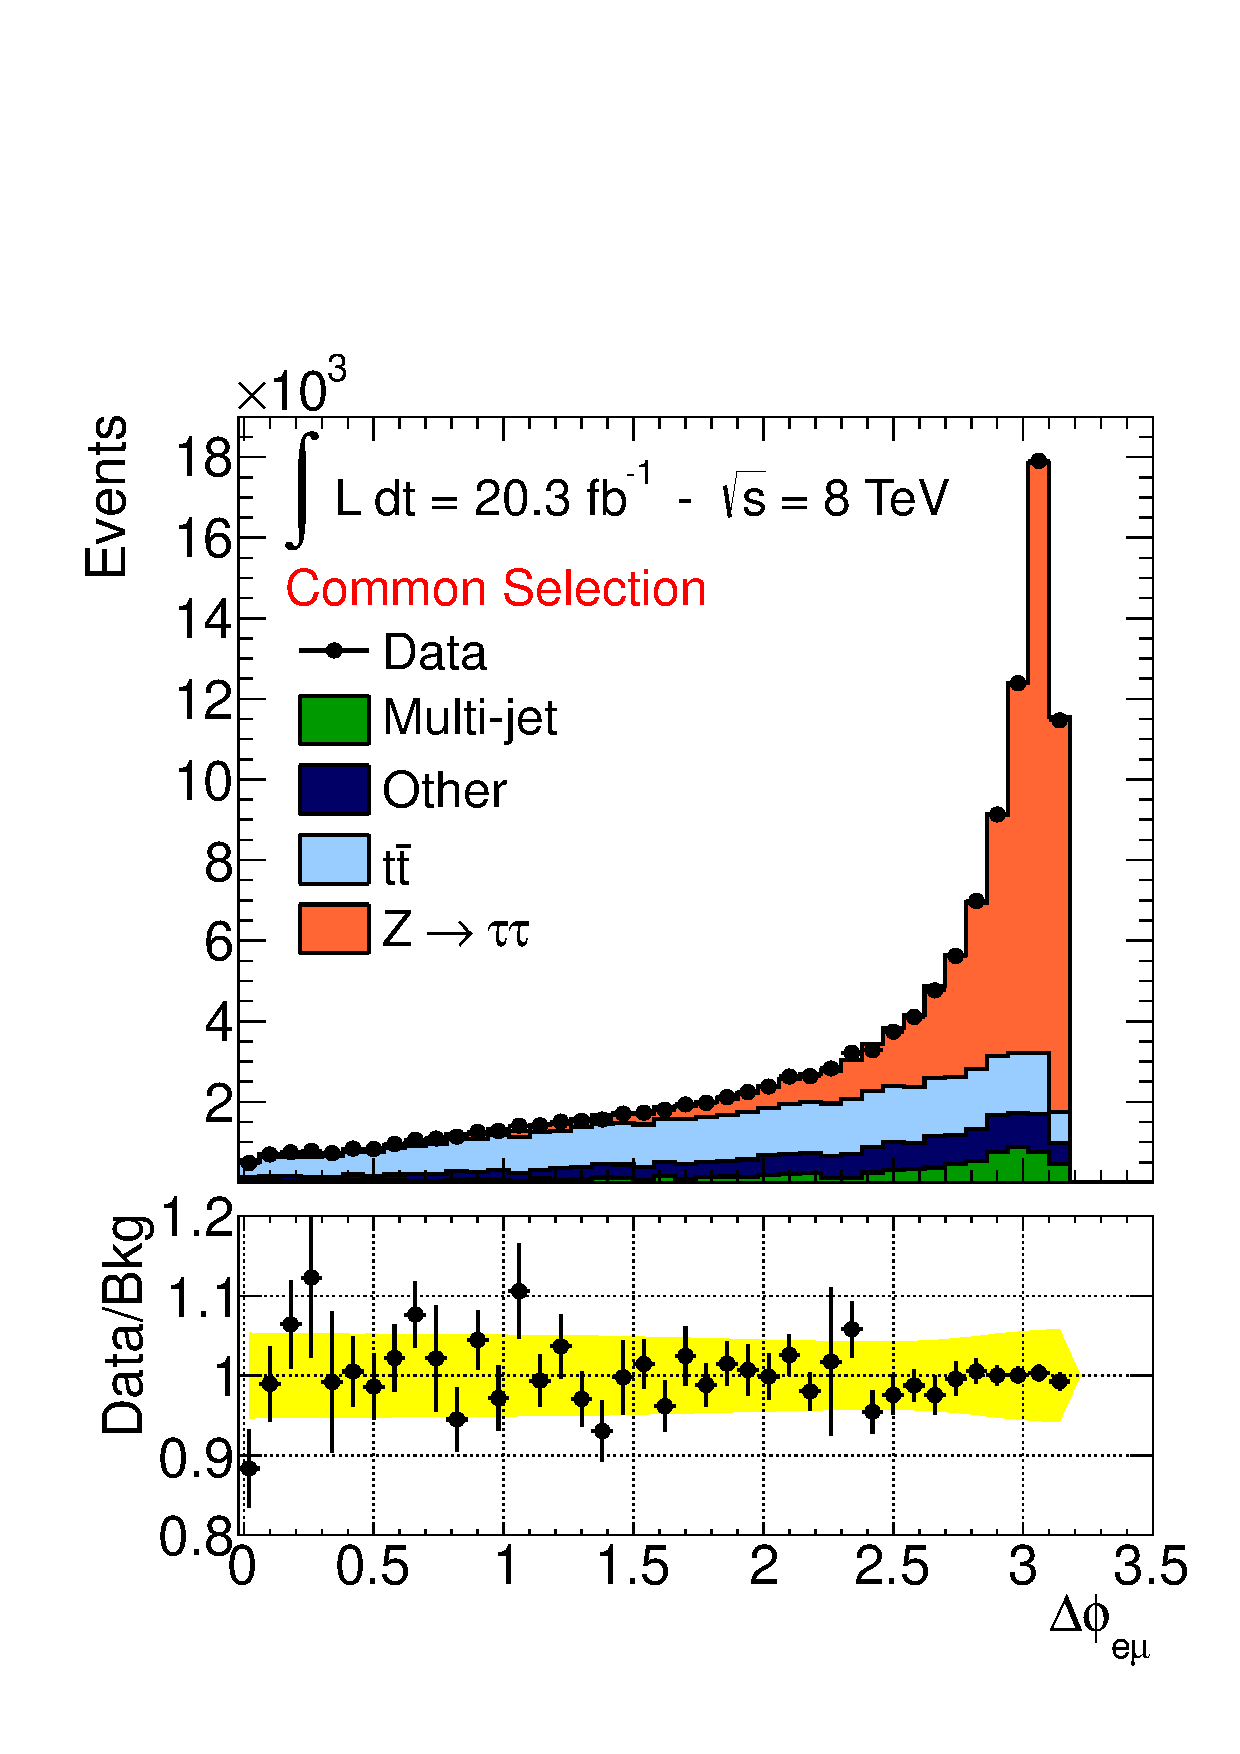
\includegraphics[width=0.47\textwidth]{figure/final_plots/std_presel_deltaPhi.pdf}
	    \label{dphi}	
     }	
     \subfigure[]{		
            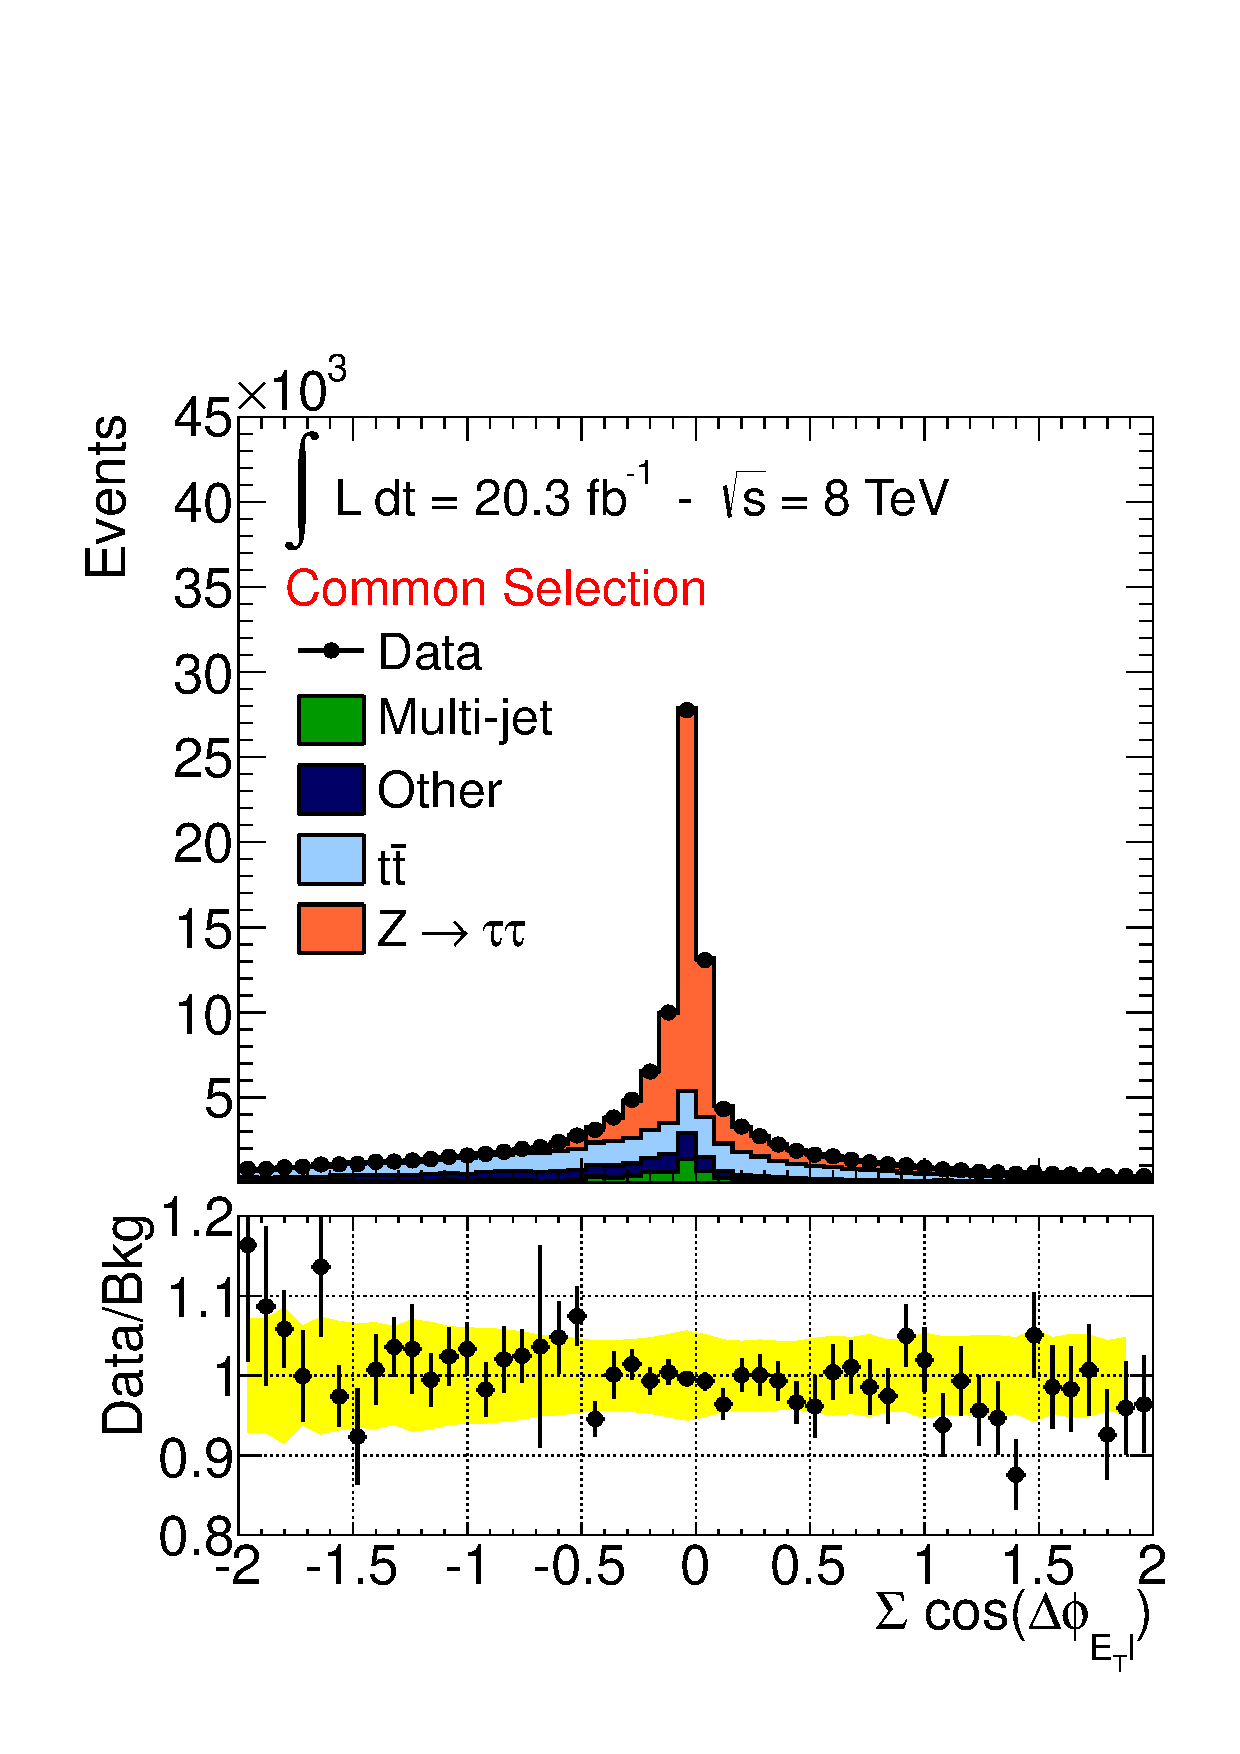
\includegraphics[width=0.47\textwidth]{figure/final_plots/std_presel_sum_cos_deltaPhi.pdf}
	    \label{sumcosphi}	
     }	
     \subfigure[]{		
            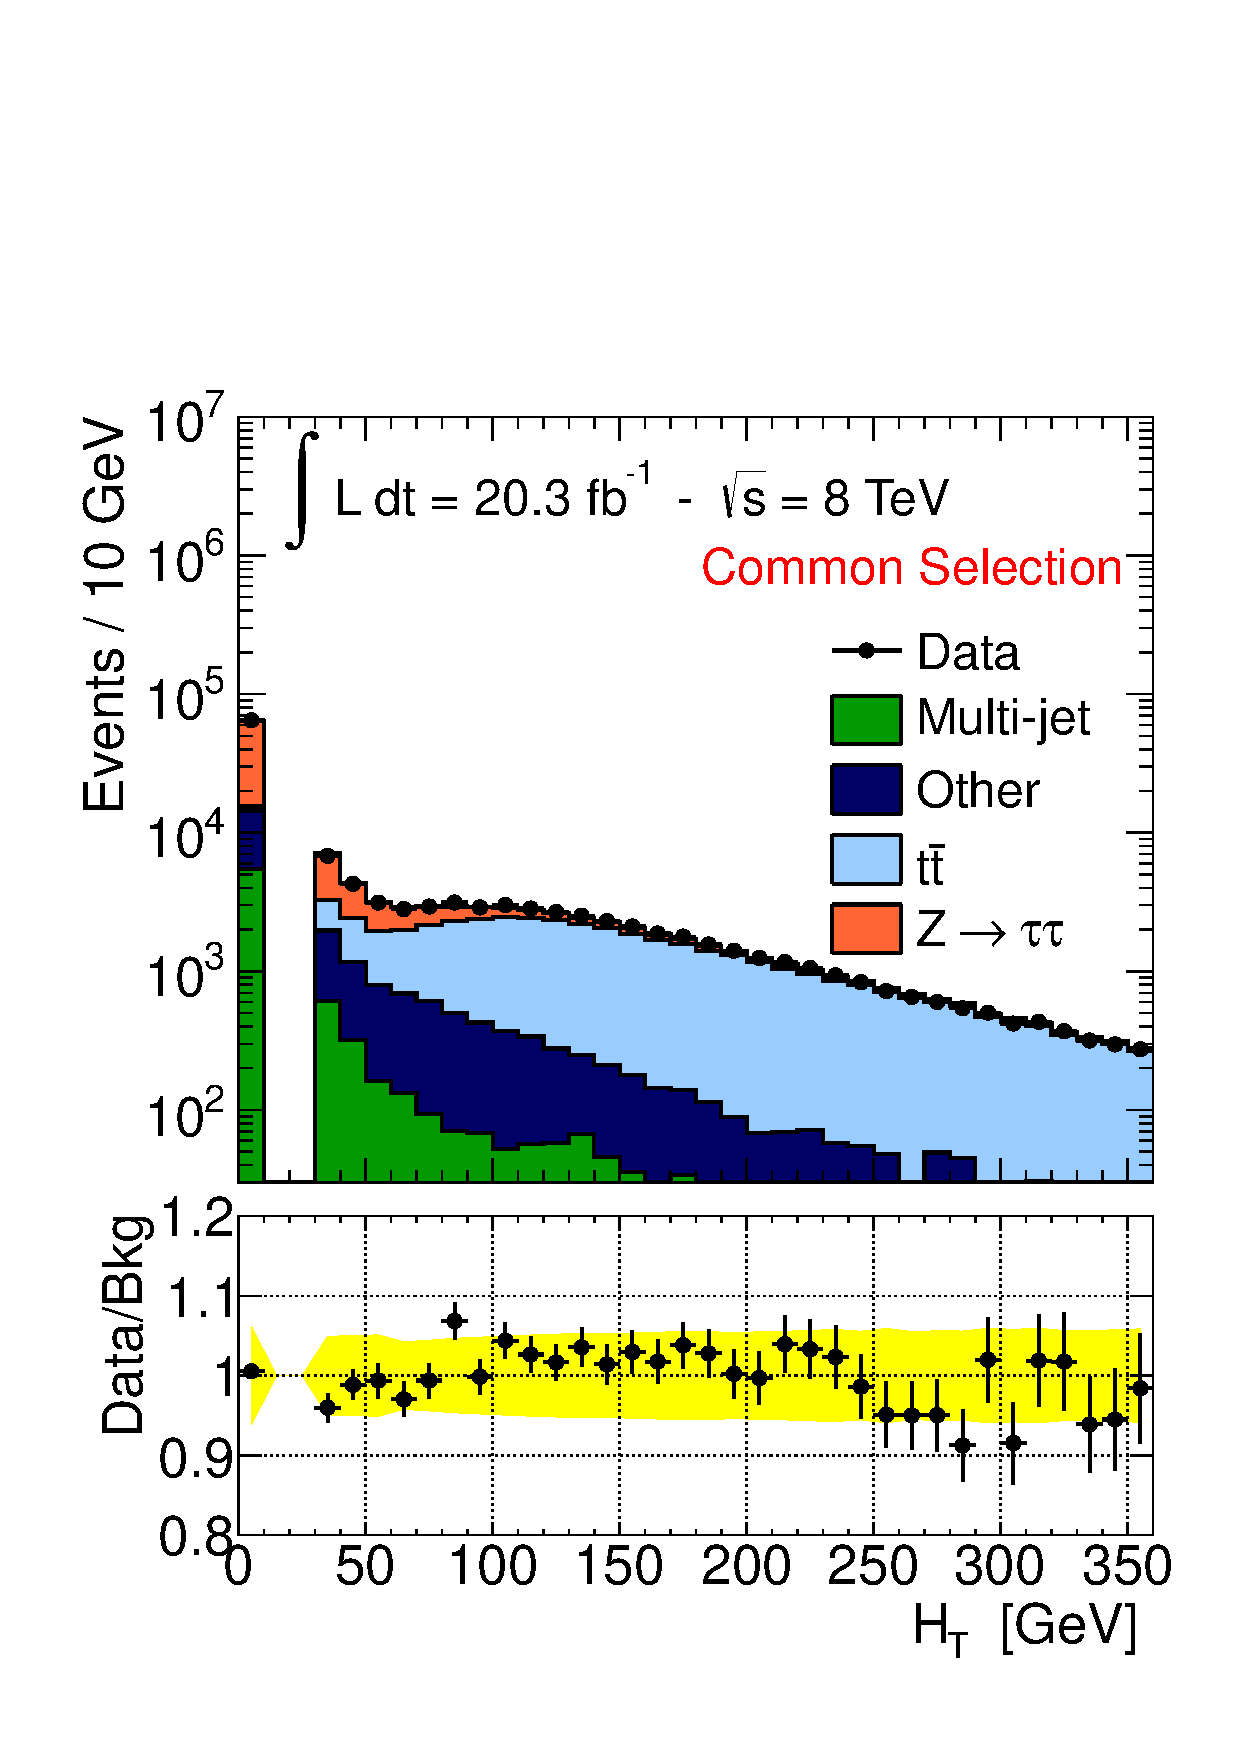
\includegraphics[width=0.47\textwidth]{figure/final_plots/std_presel_Ht.pdf}
	    \label{Ht}	
     }	
     \subfigure[]{		
            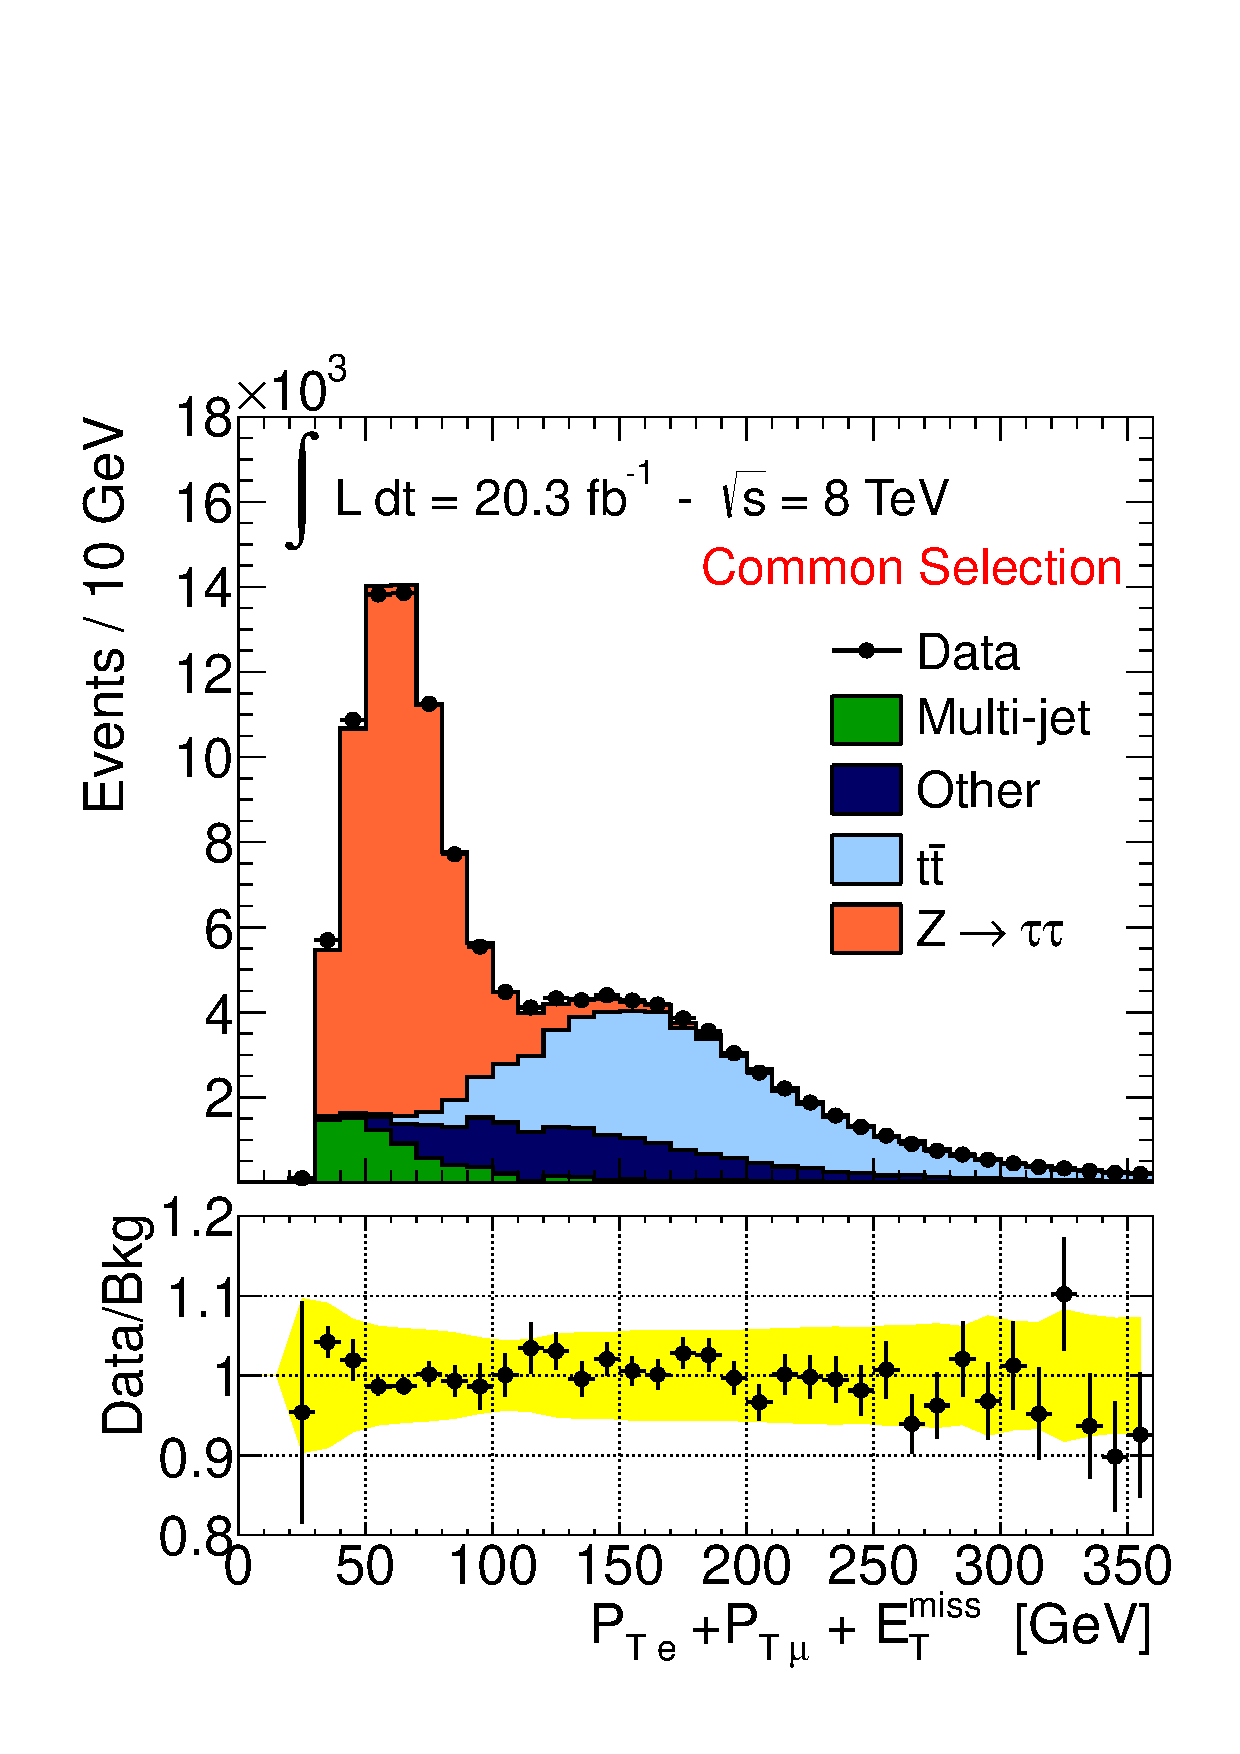
\includegraphics[width=0.47\textwidth]{figure/final_plots/std_presel_Et_plus_leptonPt.pdf}
	    \label{sumlepPt}	
     }	

    \end{center}
    \caption{Distributions of relevant discriminating variables shown after the common selection has been applied.
	The prediction of the  background model is compared to  data.
	The contribution of the $\Ztautau$ and QCD multi-jet background processes is measured in  dedicated  signal-depleted control data samples,
	the prediction for all the other bakground processes is obtained from simulation.
 	 The notation ``Other'' stands 	for the electroweak processes $\Wlnu$, $\Zll$, diboson and single top quark production.
	The yellow band represents the total systematic uncertainty for the background model prediction (see Section~\ref{sec:Systematics}).}
   \label{fig:selections}
\end{figure}

\subsection{b-tagged Event Category}\label{sec:tag}
The request of exactly one b-tagged jet in the b-tagged event category selects predominantly signal events produced 
in  b-quarks associated production mode.
Background processes with b-jet activity, as the top quark and single top quark production become enhanced compared to the $\Ztautau$ background.
Also in this category selection requirement on $\Delta\phi_{e,\mu}$ and $\sum\cos\Delta\phi$  are imposed to reduce the top quark and diboson background contributions,
as described for the b-vetoed event category. Further selection criteria specific for  this category
are employed  as described below.

Signal events in this event category can be discriminated from the top quark process given their relatively low jet activity. 
The top quark process is very likely to have two or more highly enegetic jets in the event, unlike the signal
b-jet which are relatively low energetic.
Weak jet activity is ensured by requesting the sum of the jets transverse momenta $H_T$  in the event to be small.
The $H_T$ distribution is shown in Figure~\ref{Ht}. The jets used for the calculation of the $H_T$ value 
should have $\pt > 30 $ GeV, $|\eta| < 4.5$  and $\text{JVF} > 0.5 $ (if $|\eta| < 2.5$).

Another feature that discriminate top quark  pair production from the Higgs boson signal is the higher invariant mass of the former final state, 
as the highest Higgs mass considered for the presented  search is 300 GeV.
The sum of electron and muon transverse momenta with \met is  used as 
a corresponding discriminating variable, whose distribiution is shown in Figure~\ref{sumlepPt}$\,.$

The summary of the exact optimized selection criteria for the b-tagged event category is shown in Table~\ref{tab:sel}.
In Table~\ref{tab:eventsel:btag} the predicted number of background and signal events after each stage of selection 
in the b-tagged event category  is reported.






\subsection{Mass Reconstruction with MMC Technique}\label{sec:mmc}

Acurate invariant mass reconstruction of a di-$\tau$ resonace is a challenging task due to the undetected neutrinos. 
In the presented analysis a total of four neutrinos are involved in the final state, two for each 
of the $\tau$ lepton decays.
% In case of leptonic decay of the $\tau$ leptons
%a total of four neutrinos are involved in the final state. 
The invariant mass depends on eight uknowns given by the two
sums of neutrino four-momenta, one for each $\tau$ lepton decay. These unknowns can be constrained by four parameters 
obtained from the measured  missing transverse energy and from the $\tau$ lepton mass using the following equations:
% 
%In case of leptonic decay of both $\tau$ leptons a pair of neutrinos for each
%of them are involved in the final state,  the system presents then eight unknowns, which corresponds to the four-momentum of the neutrinos pairs.
%Four additional kinematic constraint are set by the following equations:
%There are four additional constraint 
%which come from the measurement of \MET and from the fact that each single decay should have invariant mass equal to the tau mass:
\begin{equation} \label{eq:MMC}
\begin{split}
%\begin{align}
%\begin{gather*}  
&\vec{E}_T^{miss} = \vec{P}_{T}^{mis_{1}} +  \vec{P}_{T}^{mis_2} \\
&M_{\tau_{i}}^2 = m^2_{mis_{i}} + m^2_{vis_{i}} + 2 \mathbf{P}_{vis_i} \cdot \mathbf{P}_{mis_i} \\
%\end{align}
%\end{gather*}
\end{split}
\end{equation}
where the index \emph{i} runs over the two $\tau$ leptons in the event. 
$\vec{P}_{T}^{mis_{i}}$, $m_{mis_{i}}$ and $\mathbf{P}_{mis_{i}}$ are respectively the transverse momentum, the invariant mass and 
the four momentum of the pair of neutrinos originating from the decay of the $i$-th  $\tau$ 
lepton with mass $M_{\tau}$. The subscript \emph{vis} indicates instead 
quantities related to the charged lepton from  the corresponding $\tau$ lepton decay. The remaining four degrees of freedom can be 
further constrained, for example, assuming that the neutrinos are collinear to the electron or muon from the corresponding 
$\tau$ lepton decay. This approximation, however, introduces limitations on the mass resolution.

\begin{table}[!tp]
  \centering
   \begin{footnotesize}	
  \begin{tabular}{ccccc}
    \hline\hline
	&	Common Selections			&	n(b-jet)=0			&	$\Delta\phi(e-\mu)>1.6$			&	$\sum\cos\Delta\phi > -0.4$ 		\\	
    \hline
   \hline
Data	&	125886			&	89155			&	-			&	-				-			\\
   \hline
Multi-jet	&	6693	$\pm$	456	&	6357	$\pm$	461	&	5322	$\pm$	438	&	4137	$\pm$	339	\\
\Zll 	&	569	$\pm$	48	&	564	$\pm$	48	&	516	$\pm$	47	&	434	$\pm$	44		\\
\Wlnu	&	1625	$\pm$	155	&	1604	$\pm$	155	&	1145	$\pm$	125	&	714	$\pm$	101		\\
Dibosons	&	9338	$\pm$	48	&	9235	$\pm$	48	&	7358	$\pm$	43	&	4002	$\pm$	31		\\
\ttbar	&	40632	$\pm$	106	&	7707	$\pm$	46	&	5044	$\pm$	37	&	3416	$\pm$	31		\\
Single Top	&	4449	$\pm$	44	&	1664	$\pm$	27	&	1124	$\pm$	22	&	682	$\pm$	18	\\
\Ztautau	&	61503	$\pm$	68	&	60440	$\pm$	67	&	58078	$\pm$	65	&	55303	$\pm$	64	\\
%Signal	&				&				&	-			&	-						\\
    \hline
  \end{tabular}
  \caption{Number of observed and predicted signal and background events, after each selection stage in the b-vetoed event category.}
  \label{tab:eventsel:bveto}
   \end{footnotesize}	
\end{table}

\begin{table}[!t]
  \centering
   \begin{footnotesize}	
  \begin{tabular}{cccccccc}
    \hline\hline
	& 	n(b-jet)=1			&	$\Delta\phi$&	$\sum\cos\Delta\phi$			&	$P_{T\mu} + P_{Te} + \met$&	$ H_T$	\\
   \hline
Data	&	23352			&	-			&	-			&	-			&	-						\\
   \hline
Multi-jet	330	$\pm$	40	&	208	$\pm$	27	&	135	$\pm$	22	&	114	$\pm$	17	&	100	$\pm$	15	\\
\Zll 	&	5.2	$\pm$	1.8	&	2.3	$\pm$	1.1	&	2.3	$\pm$	1.1	&	1.7	$\pm$	1.0	&	0.9	$\pm$	0.8		\\
\Wlnu	&	20	$\pm$	6	&	15	$\pm$	6	&	13	$\pm$	6	&	10	$\pm$	6	&	10	$\pm$	6		\\
Dibosons	&	99	$\pm$	5	&	63	$\pm$	4	&	36.4	$\pm$	3.0	&	14.8	$\pm$	1.8	&	13.3	$\pm$	1.8		\\
\ttbar	&	19810	$\pm$	70	&	9680	$\pm$	50	&	6450	$\pm$	50	&	808	$\pm$	15	&	350	$\pm$	10		\\
Single Top &	2456	$\pm$	33	&	1223	$\pm$	23	&	784	$\pm$	18	&	122	$\pm$	7	&	99	$\pm$	7		\\
\Ztautau &	952	$\pm$	9	&	625	$\pm$	7	&	540	$\pm$	7	&	482	$\pm$	6	&	421	$\pm$	6		\\
%Signal		&				&	-			&	-			&	-			&	-						\\
    \hline
    \hline
  \end{tabular}
  \caption{Number of observed and predicted signal and background events, after each selection stage in the b-tagged event category.}
  \label{tab:eventsel:btag}
   \end{footnotesize}	
\end{table}  %INCOMPLETE ------------missing signal

In this analysis, the so-called "Missing Mass Calculator" (MMC) algorithm
is used to calculate the most likely  invariant mass of the di-$\tau$ system for a given event topology. %event kinematics
The implementation of the MMC method in this search is based on~\cite{MMC}. 
The MMC algorithm solves the equations~\ref{eq:MMC} for a set of points in a grid of a 
%assigning values to the yet undetermined variables, performing a ``scan'' over a 
four-dimensional parameter space. The four independent  variables are chosen 
to be $ m^2_{mis_{i}}$ and $cos\theta^*_i$ , the latter defined
as the angle between the charged lepton from the $\tau$ lepton decay and the boost direction of the $\tau$ lepton. 
The di-$\tau$ invariant mass in each  event is then  calculated for each given point of the parameter space.
Each solution is weighted by the probability that a $\tau$ lepton decay assumes a given configuration. The probability
of a given configuration is predicted  by means of simulation using PYTHIA generator supplemented with TAUOLA package. 
The invariant mass of the di-$\tau$  system, \mmc, is then defined as the maximum of the weighted invariant 
mass distribution obtained from all scanned points.

\begin{figure}[p]
     \begin{center}
     \subfigure[]{		
            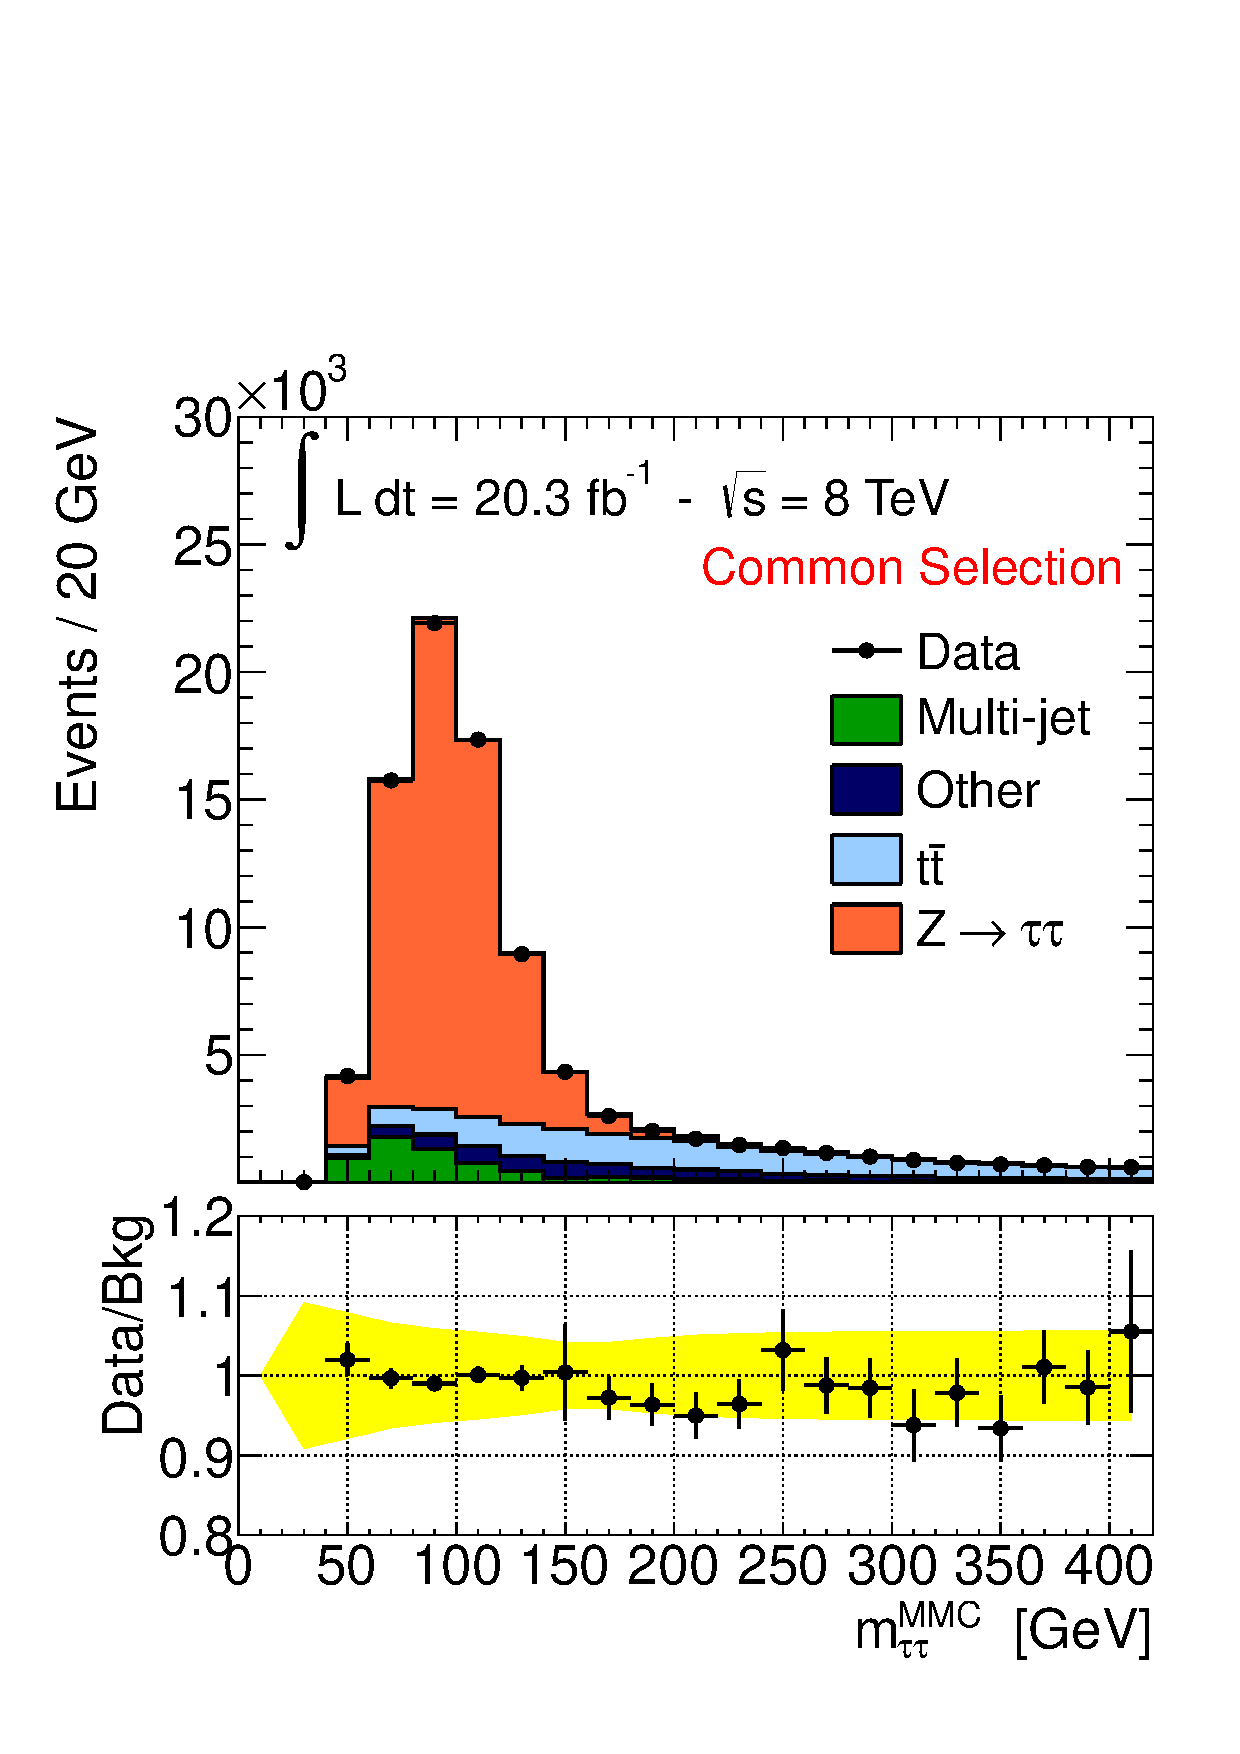
\includegraphics[width=0.47\textwidth]{figure/final_plots/std_presel_mmc_mass.pdf}
     }	
     \subfigure[]{		
            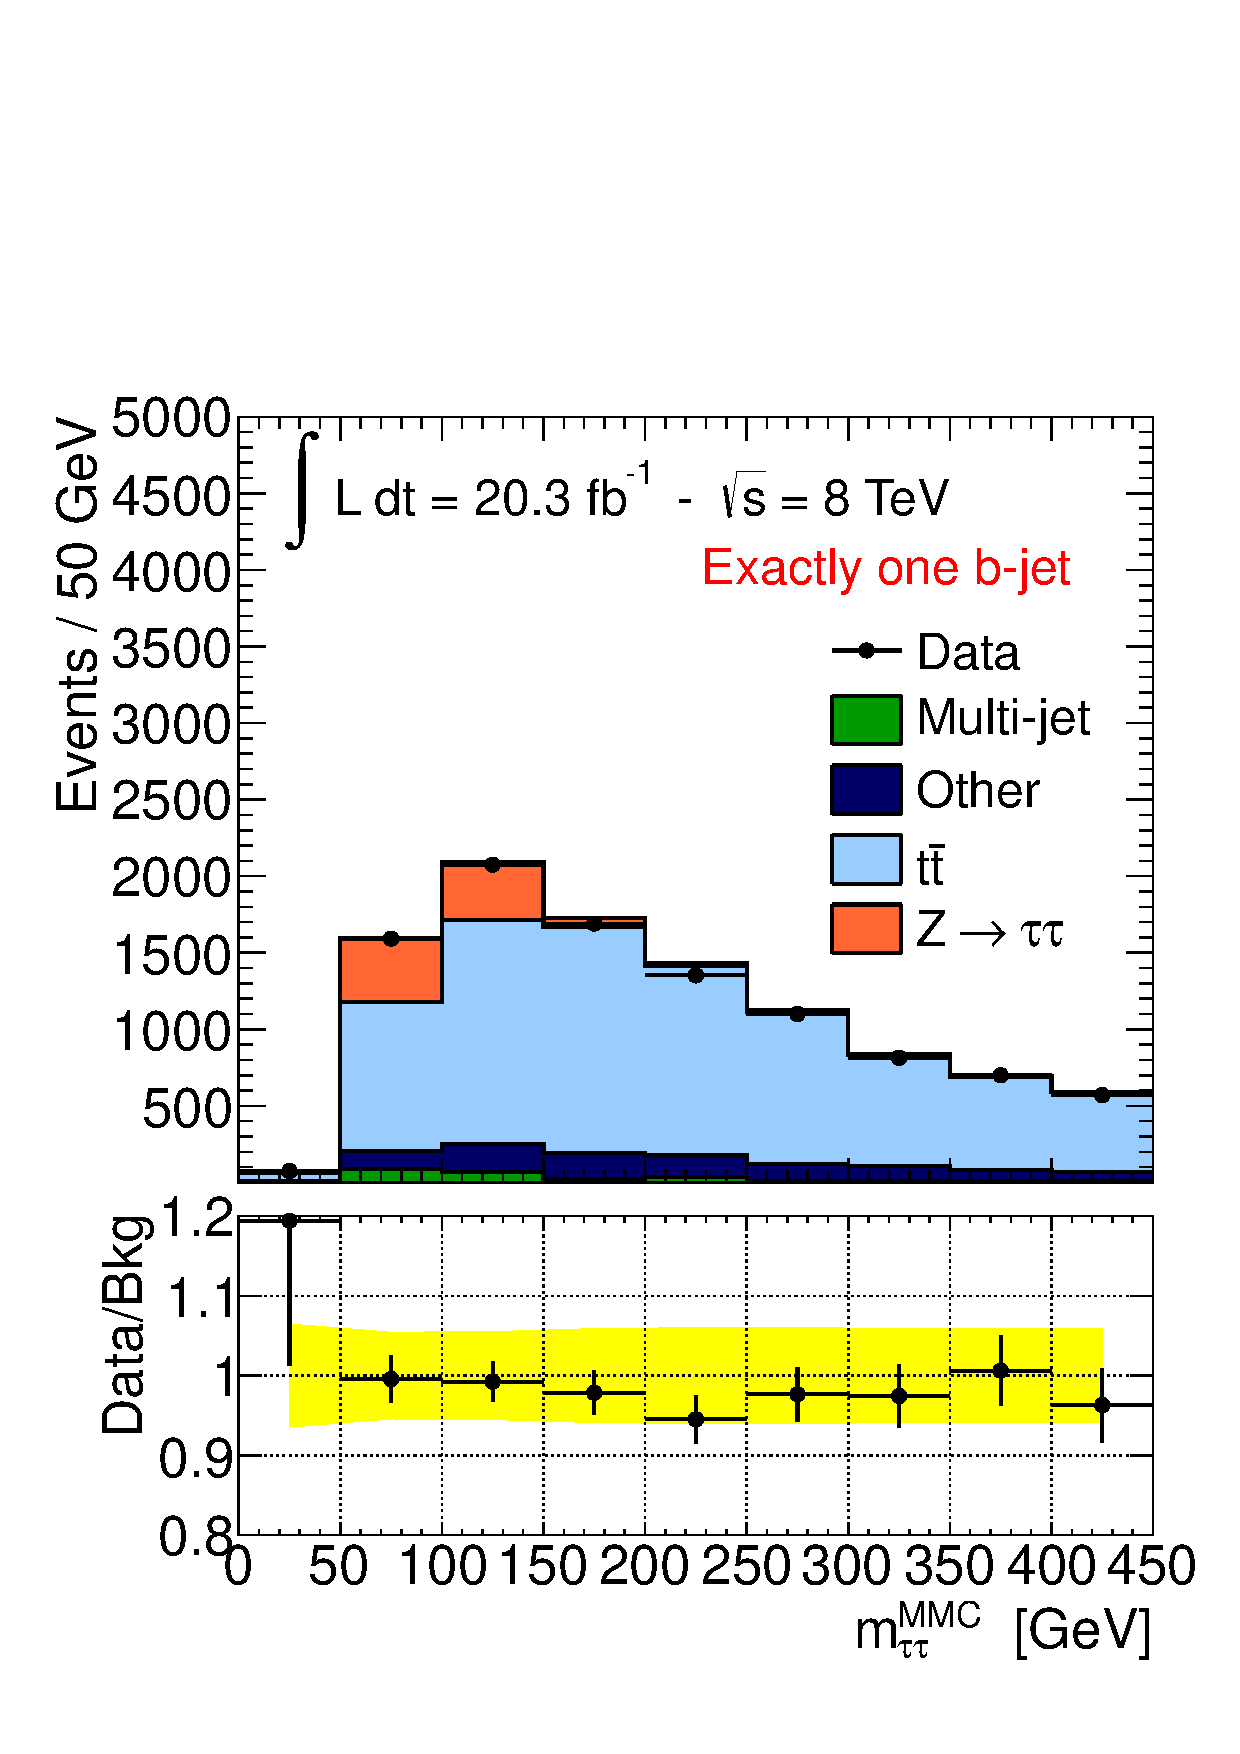
\includegraphics[width=0.47\textwidth]{figure/final_plots/std_presel_Btag_mmc_mass.pdf}
     }	
     \subfigure[]{		
            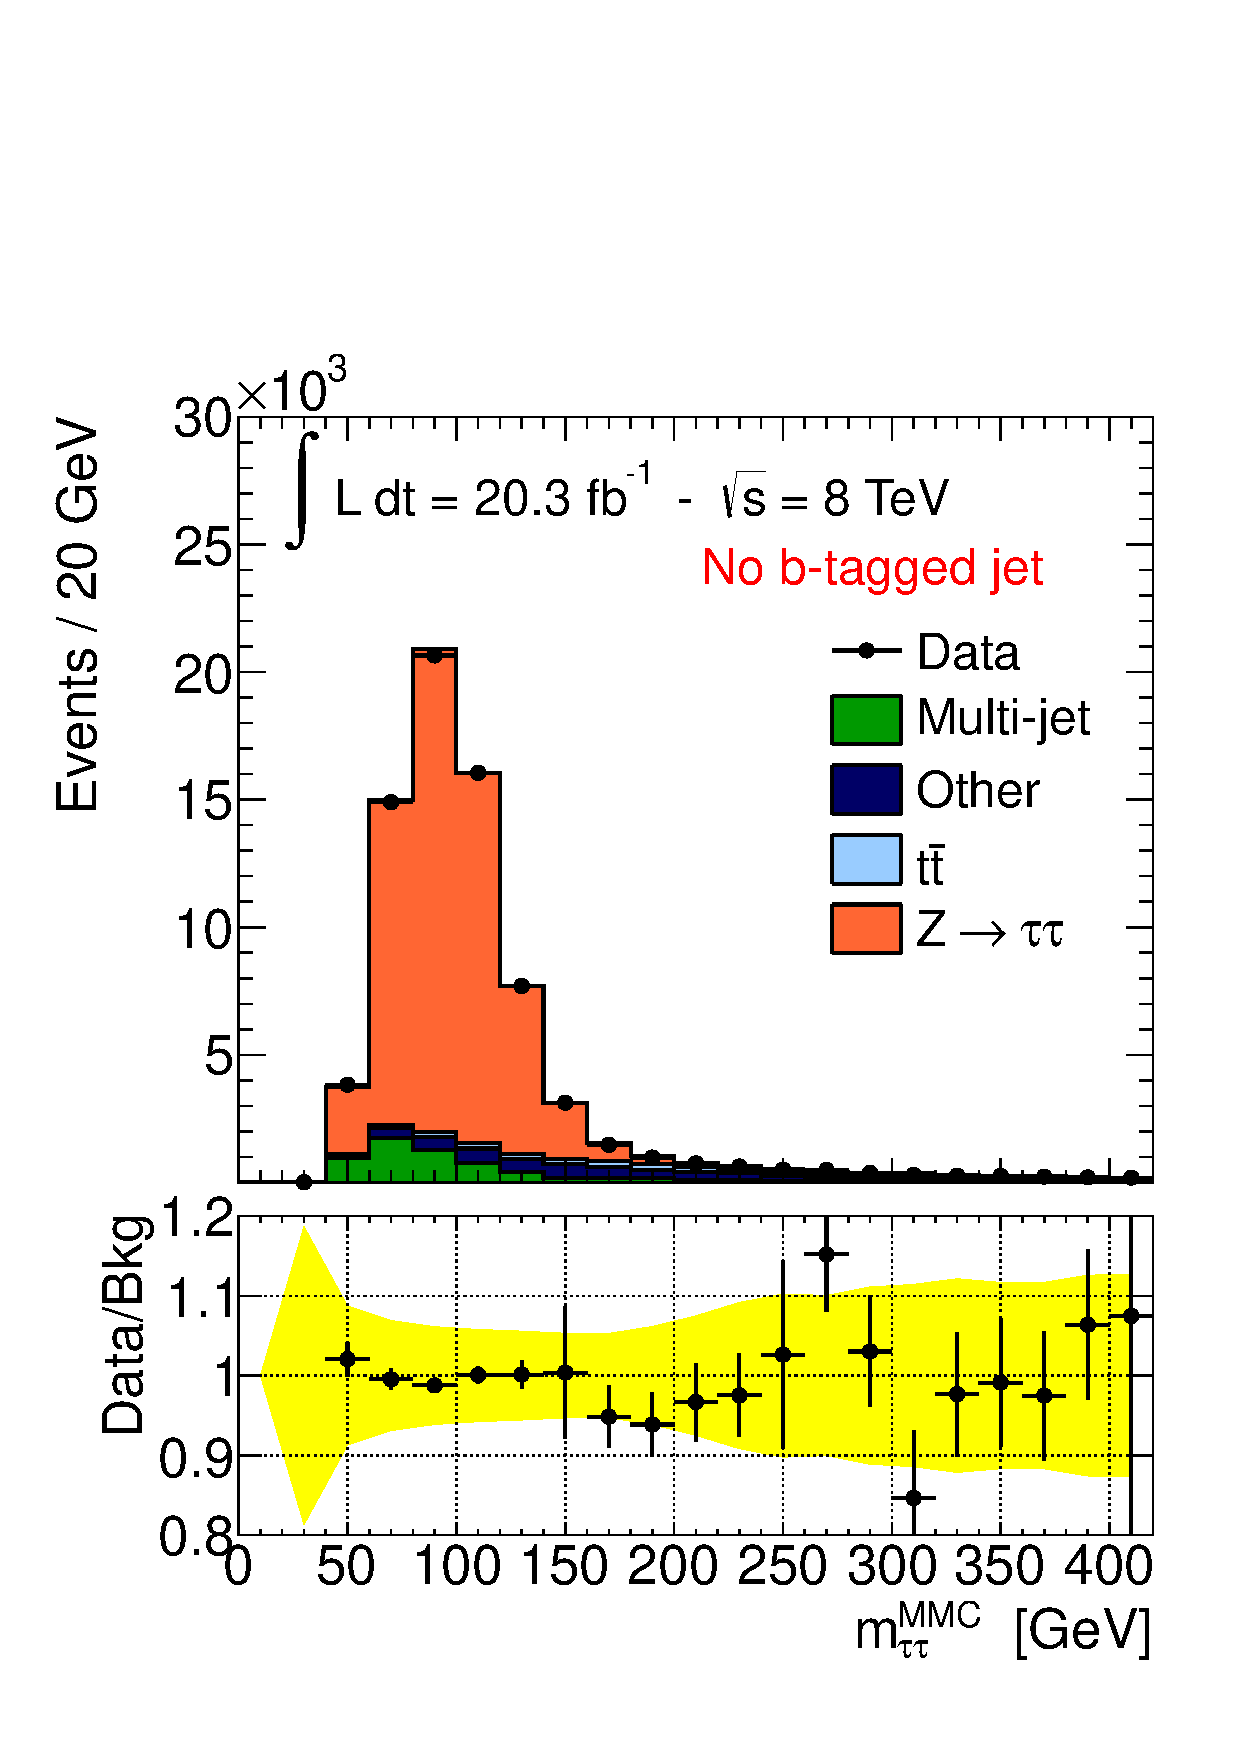
\includegraphics[width=0.47\textwidth]{figure/final_plots/std_presel_NoBtag_mmc_mass.pdf}
     }	
%     \subfigure[]{		
%            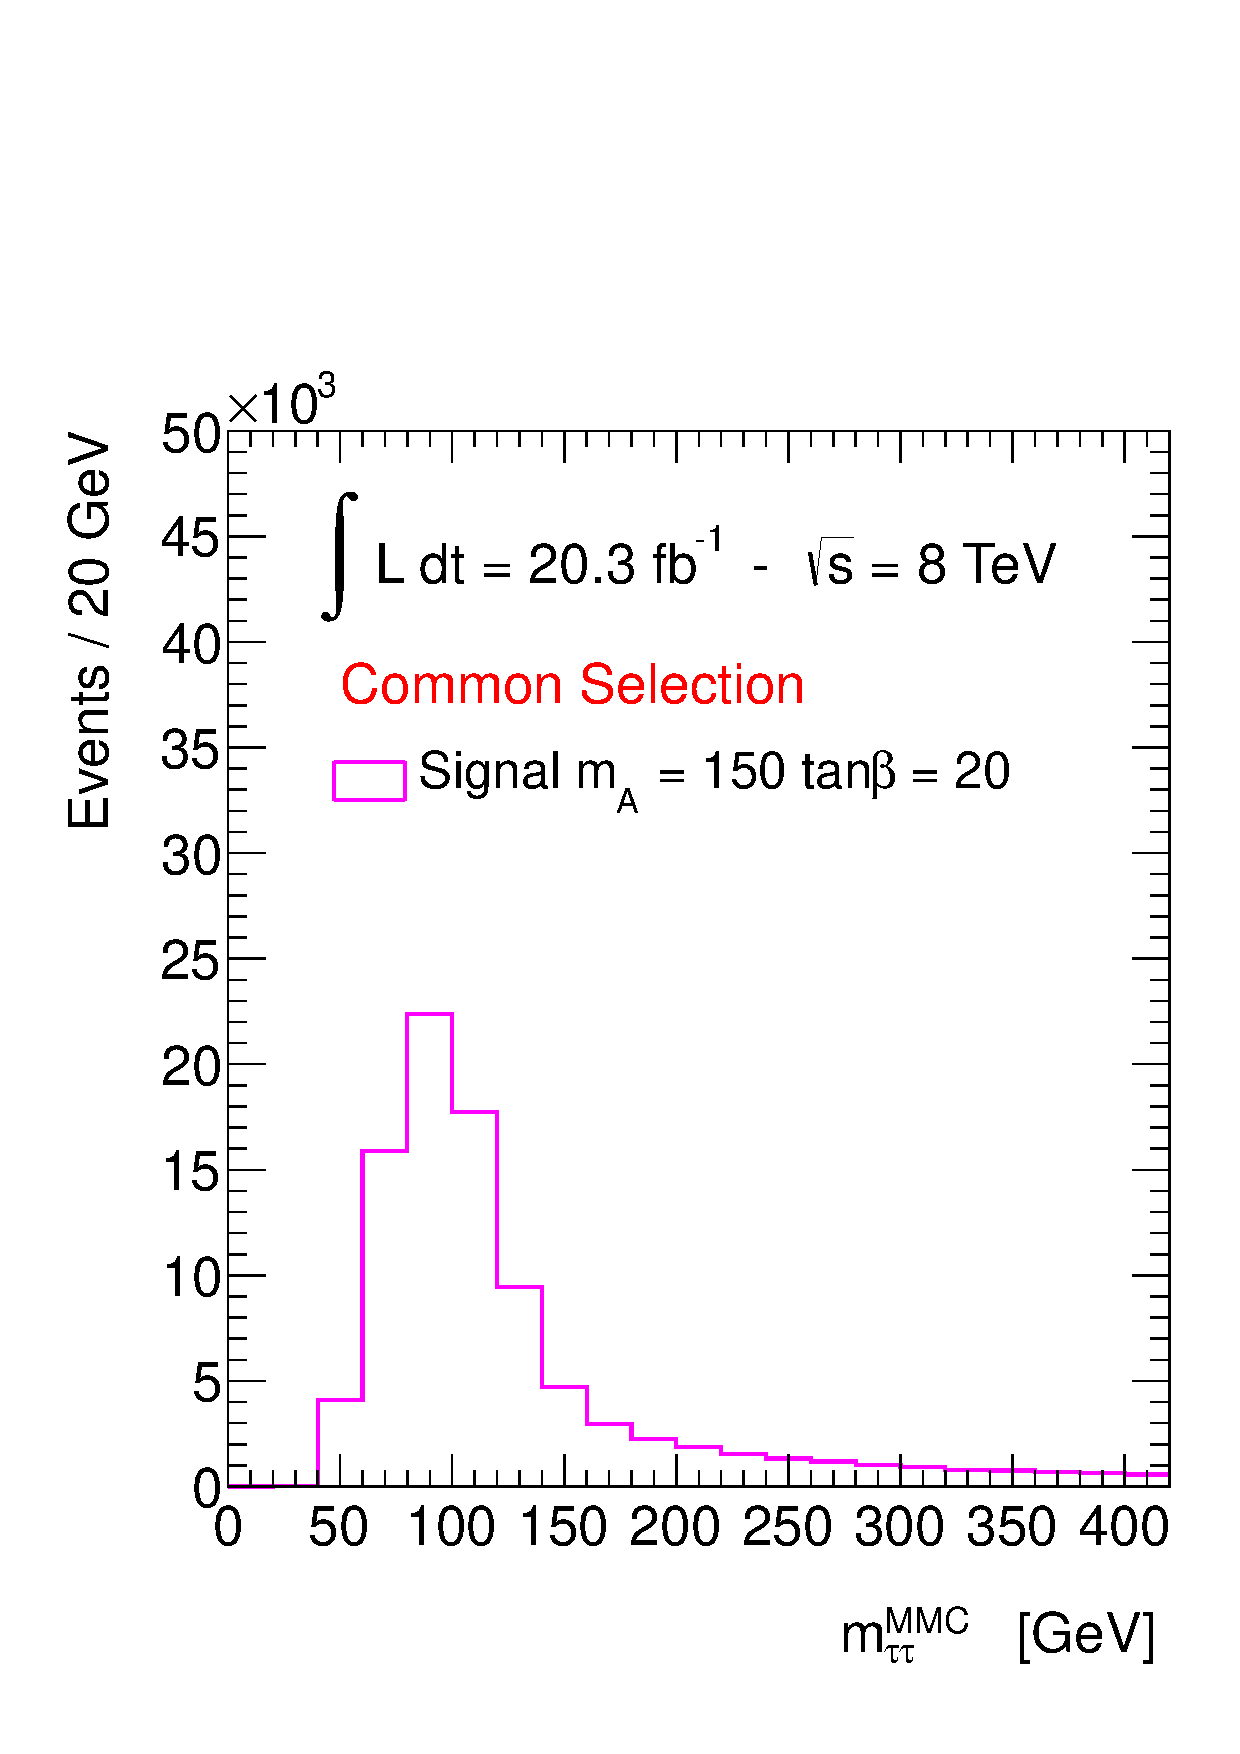
\includegraphics[width=0.47\textwidth]{figure/final_plots/signal_presel.pdf}
%     }	

    \end{center}
     	

    \caption{Observed and expected distribution of the 
	invariant di-$\tau$ mass \mmc for different stage of analysis selections: after requiring the common selection (a),
	additionally requiring the presence of exactly one b-tagged jet (b) or the absence of a b-tagged jet (c).
	The prediction of the  background model is compared to  data.
        The contribution of the $\Ztautau$ and QCD multi-jet background processes is measured in  dedicated  signal-depleted control data samples,
        the prediction for all the other background processes is obtained from simulation.
        The notation ``Other'' stands  for the electroweak processes $\Wlnu$, $\Zll$, diboson and single top quark production.
        The yellow band represents the total systematic uncertainty for the background model prediction.}
   \label{fig:mass}
\end{figure}


The resolution of the missing transverse energy measurement impacts the resolution of the invariant mass obtained with the \mmc method.
To improve the $\met$ resolution, a scan over a six-dimensional parameter space is performed 
in a similar manner as described above. For this purpose, the value of $\vec{E}_T^{miss}$ is also considered unknown and a scan 
is performed over all possible values constrained by the measured $\met$ and its corresponding uncertainty.
%on it assigning values  according to its uncertainty. 
%The probability of each solution is calculated and the final missing transverse
%energy is given by the weighted mean of the scanned points. 
%
%The final procedure consist in obtaining first an estimate for $\met$ by means of a six dimensional scan over the solution of equations~\ref{eq:MMC},
%successively a four dimensional scan is performed fixing $\met$ to the updated value and calculating the most likely invariant mass 
%of the di-$\tau$ system.

Figure~\ref{fig:mass} shows the  \mmc invariant mass distribution after the common selection and after the requirement of the presence or the
absence of a b-tagged jet.

 
%Accurate invariant mass reconstruction of a di-tau system is a challenging task due to the escaping neutrinos.
%In this analysis, with four neutrinos in the final state, the number of unknown largely exceed the number of constraints,
%several approximation are possible to further constraint the neutrinos, for example assuming them collinear to the 
%other leptons from tau decay, however those approximation suffers of limitations. 

%In this analysis we use the so called missing mass calculator (MMC)~\cite{MMC}
%technique for the calculation of the di-tau system invariant mass. This technique employs additional 
%information from the well known tau decay to constraint the system, this is achieved by minimising a likelihood function 
%defined in the kinematically allowed phase space region, the result is a more precise measurement of the di-tau 
%system invariant mass and a considerable improvement in resolution. The invariant mass distribution 
%calculated with the MMC technique is referred in the following as $\mmc$ and is used as discriminating 
%variable in the limits setting.

